\documentclass{tufte-handout}

%\geometry{showframe}% for debugging purposes -- displays the margins

\usepackage{amsmath}

% Set up the images/graphics package
\usepackage{graphicx}
\setkeys{Gin}{width=\linewidth,totalheight=\textheight,keepaspectratio}
\graphicspath{{graphics/}}

\title{Physics stuff}
\author{Alex Weatherall}
%\date{24 January 2009}  % if the \date{} command is left out, the current date will be used

% The following package makes prettier tables.  We're all about the bling!
\usepackage{booktabs}

% The units package provides nice, non-stacked fractions and better spacing
% for units.
\usepackage{units}

% The fancyvrb package lets us customize the formatting of verbatim
% environments.  We use a slightly smaller font.
\usepackage{fancyvrb}
\fvset{fontsize=\normalsize}

% Small sections of multiple columns
\usepackage{multicol}

% Provides paragraphs of dummy text
\usepackage{lipsum}

% These commands are used to pretty-print LaTeX commands
\newcommand{\doccmd}[1]{\texttt{\textbackslash#1}}% command name -- adds backslash automatically
\newcommand{\docopt}[1]{\ensuremath{\langle}\textrm{\textit{#1}}\ensuremath{\rangle}}% optional command argument
\newcommand{\docarg}[1]{\textrm{\textit{#1}}}% (required) command argument
\newenvironment{docspec}{\begin{quote}\noindent}{\end{quote}}% command specification environment
\newcommand{\docenv}[1]{\textsf{#1}}% environment name
\newcommand{\docpkg}[1]{\texttt{#1}}% package name
\newcommand{\doccls}[1]{\texttt{#1}}% document class name
\newcommand{\docclsopt}[1]{\texttt{#1}}% document class option name

\begin{document}

\maketitle% this prints the handout title, author, and date

\begin{abstract}
\noindent This topic covers the basics of Physics! Mechanics and stuff etc.
\end{abstract}

\section{Learning Objectives}
By the end of this topic you should be able to:
\begin{itemize}
\item State something
\item Explain something
\item Compare something
\end{itemize}

\pagebreak

\section{Topic 1}

\newthought{A major advantage of Physics}, is that it is \textit{AwESomE}\sidenote{It really really is.}, and I think I'm going to be able to use LateX to produce my notes.

\subsection{Sub topic 1}

There are hundreds, if not thousands of things to learn. There are hundreds, if not thousands of things to learn. There are hundreds, if not thousands of things to learn. There are hundreds, if not thousands of things to learn. There are hundreds, if not thousands of things to learn. There are hundreds, if not thousands of things to learn. There are hundreds, if not thousands of things to learn. There are hundreds, if not thousands of things to learn. There are hundreds, if not thousands of things to learn.  

\newthought{Physically,} physics is full of physics. (see Figure \ref{fig:figure-one}).  Often, it's also full of other stuff.

\begin{marginfigure}[0in]
  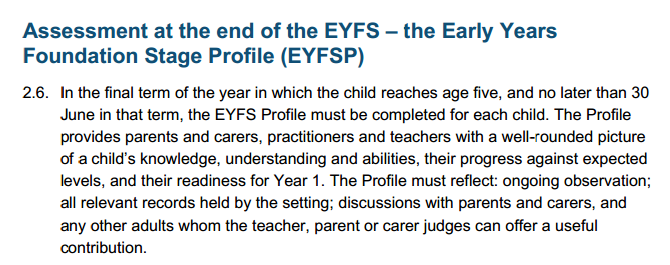
\includegraphics{figures/testimage}
  \caption{A figure of much importance.}
    \label{fig:figure-one}
\end{marginfigure}

\newthought{Some more stuff,} can be written about other bits and pieces. (see Table \ref{tab:table-one}).

\begin{margintable}
  \centering
  \begin{tabular}{lll}
    \toprule
    Voltage / V & Current / I & Resistance / $\Omega$ \\
    \midrule
    1.0 & 2.0 & 0.5 \\
    2.0 & 4.0 & 0.5 \\
    3.0 & 6.0 & 0.5 \\
    \bottomrule
  \end{tabular}
  \caption{Resistance is futile}
  \label{tab:table-one}
  %\zsavepos{pos:normaltab}
\end{margintable}

\newthought{Functionally,} I need to remember to \emph{emphasise}  some examples. 

\section{Another Topic}
\subsection{Sub topic 1}
\subsection{Sub Topic 2}

\newthought{The force\sidenote{due to the acceleration}} this is a thing to be reckoned with. (see Table \ref{tab:forces}):

\begin{table}
  \centering
  \begin{tabular}{lcl}
    \toprule
    Force & Particle & Affects \\
    \midrule
    strong & gluon & nucleons/quarks \\
    weak & W+, W-, Z boson & hadrons/leptons/mesons \\
    gravity & graviton & matter \\
    electromagnetic & $\gamma$ photon & charged \\
    \bottomrule
  \end{tabular}
  \caption{Some forces.}
  \label{tab:forces}
  %\zsavepos{pos:normaltab}
\end{table}

\section{Electricity}

\bibliography{library}
\bibliographystyle{plainnat}

\end{document}